\section{Referencia de la Clase Facturas\-Proveedor\-List}
\label{classFacturasProveedorList}\index{FacturasProveedorList@{FacturasProveedorList}}
Administra el listado de facturas de proveedor.  


{\tt \#include $<$facturasplist.h$>$}

Diagrama de colaboraci\'{o}n para Facturas\-Proveedor\-List:\begin{figure}[H]
\begin{center}
\leavevmode
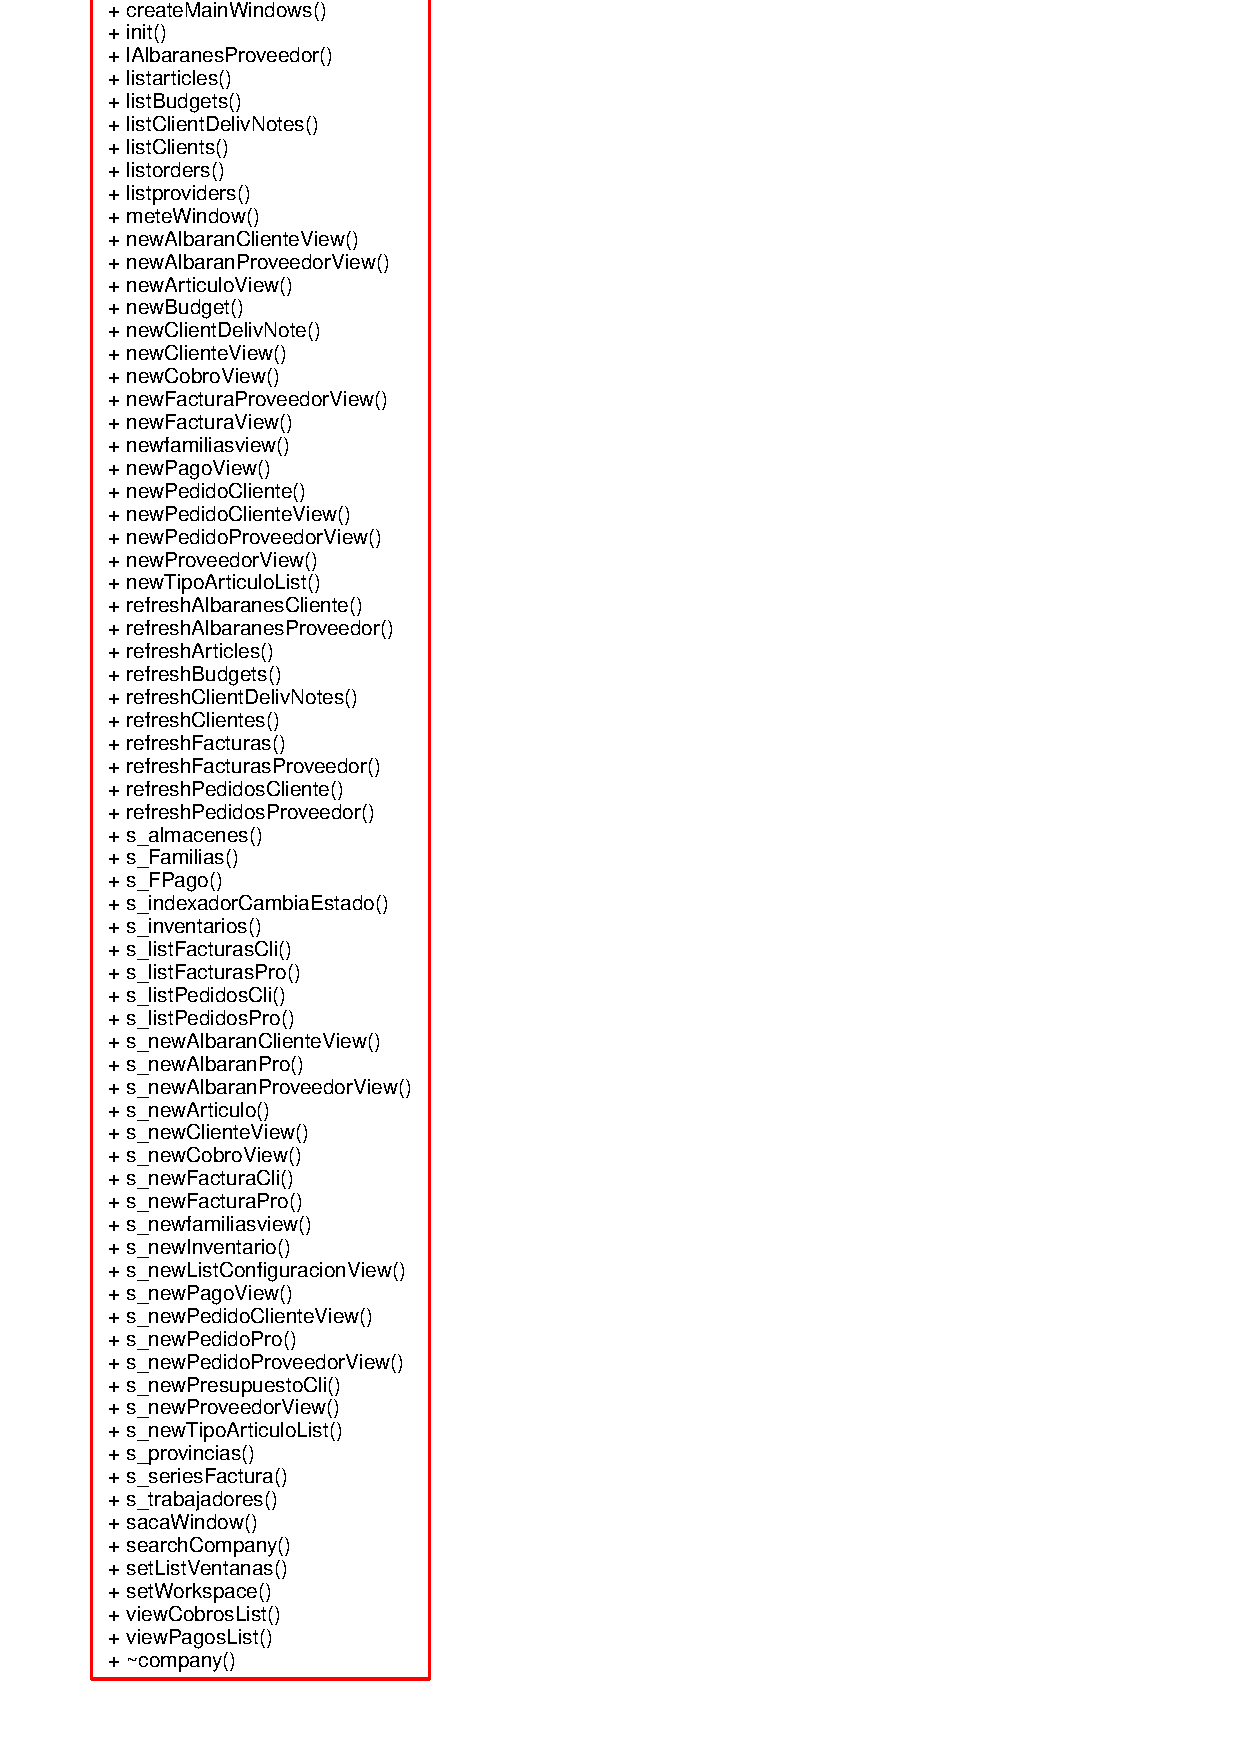
\includegraphics[width=133pt]{classFacturasProveedorList__coll__graph}
\end{center}
\end{figure}
\subsection*{Slots p\'{u}blicos}
\begin{CompactItemize}
\item 
virtual void {\bf on\_\-m\_\-filtro\_\-text\-Changed} (const QString \&text)\label{classFacturasProveedorList_i0}

\item 
virtual void {\bf on\_\-mui\_\-actualizar\_\-clicked} ()\label{classFacturasProveedorList_i1}

\item 
virtual void {\bf on\_\-mui\_\-borrar\_\-clicked} ()\label{classFacturasProveedorList_i2}

\item 
virtual void {\bf on\_\-mui\_\-configurar\_\-toggled} (bool checked)\label{classFacturasProveedorList_i3}

\item 
virtual void {\bf on\_\-mui\_\-crear\_\-clicked} ()\label{classFacturasProveedorList_i4}

\item 
virtual void {\bf on\_\-mui\_\-editar\_\-clicked} ()\label{classFacturasProveedorList_i5}

\item 
virtual void {\bf on\_\-mui\_\-imprimir\_\-clicked} ()\label{classFacturasProveedorList_i6}

\item 
void {\bf on\_\-mui\_\-list\_\-item\-Double\-Clicked} (QTable\-Widget\-Item $\ast$)\label{classFacturasProveedorList_i7}

\end{CompactItemize}
\subsection*{Se\~{n}ales}
\begin{CompactItemize}
\item 
void {\bf selected} (QString)\label{classFacturasProveedorList_l0}

\end{CompactItemize}
\subsection*{M\'{e}todos p\'{u}blicos}
\begin{CompactItemize}
\item 
void {\bf cargaconfig} ()\label{classFacturasProveedorList_a0}

\item 
void {\bf editar} (int)\label{classFacturasProveedorList_a1}

\item 
{\bf Facturas\-Proveedor\-List} ({\bf company} $\ast$, QWidget $\ast$parent=0)\label{classFacturasProveedorList_a2}

\item 
{\bf Facturas\-Proveedor\-List} (QWidget $\ast$parent=0, Qt::WFlags flag=0)\label{classFacturasProveedorList_a3}

\item 
QString {\bf genera\-Filtro} ()
\item 
void {\bf guardaconfig} ()\label{classFacturasProveedorList_a5}

\begin{CompactList}\small\item\em Funciones que se encargan de guardar y cargar la configuracion del listado. \item\end{CompactList}\item 
void {\bf hide\-Botonera} ()\label{classFacturasProveedorList_a6}

\item 
void {\bf hide\-Busqueda} ()\label{classFacturasProveedorList_a7}

\item 
QString {\bf idfacturap} ()\label{classFacturasProveedorList_a8}

\item 
void {\bf mete\-Window} (QString nom, QObject $\ast$obj)\label{classFacturasProveedorList_a9}

\item 
void {\bf modoedicion} ()\label{classFacturasProveedorList_a10}

\item 
void {\bf modoseleccion} ()\label{classFacturasProveedorList_a11}

\item 
void {\bf presenta} ()
\item 
void {\bf setcompany} ({\bf company} $\ast$comp)\label{classFacturasProveedorList_a13}

\item 
void {\bf setidarticulo} (QString val)\label{classFacturasProveedorList_a14}

\item 
void {\bf setidproveedor} (QString val)\label{classFacturasProveedorList_a15}

\item 
void {\bf show\-Botonera} ()\label{classFacturasProveedorList_a16}

\item 
void {\bf show\-Busqueda} ()\label{classFacturasProveedorList_a17}

\end{CompactItemize}


\subsection{Descripci\'{o}n detallada}
Administra el listado de facturas de proveedor. 



\subsection{Documentaci\'{o}n de las funciones miembro}
\index{FacturasProveedorList@{Facturas\-Proveedor\-List}!generaFiltro@{generaFiltro}}
\index{generaFiltro@{generaFiltro}!FacturasProveedorList@{Facturas\-Proveedor\-List}}
\subsubsection{\setlength{\rightskip}{0pt plus 5cm}QString Facturas\-Proveedor\-List::genera\-Filtro ()}\label{classFacturasProveedorList_a4}


Tratamiento de los filtros. \index{FacturasProveedorList@{Facturas\-Proveedor\-List}!presenta@{presenta}}
\index{presenta@{presenta}!FacturasProveedorList@{Facturas\-Proveedor\-List}}
\subsubsection{\setlength{\rightskip}{0pt plus 5cm}void Facturas\-Proveedor\-List::presenta ()}\label{classFacturasProveedorList_a12}


Hacemos el calculo del total. 

La documentaci\'{o}n para esta clase fu\'{e} generada a partir de los siguientes archivos:\begin{CompactItemize}
\item 
facturasplist.h\item 
facturasplist.cpp\end{CompactItemize}
